\documentclass[12pt,letterpaper]{article}
\usepackage{bbm}
\usepackage[multiple]{footmisc}
\usepackage{floatpag,amsmath,amsthm,amssymb}
%\usepackage{subcaption} 
\newtheorem{proposition}{Proposition}
\numberwithin{equation}{section}
\newtheorem{nono-prop}{Proposition}[]

%%%%%%%%%%%%%%%%%%%%%%%%%%%%%%%
%% LOAD LOCAL COMPILATION PATHS
%%%%%%%%%%%%%%%%%%%%%%%%%%%%%%%
\newcommand{\HOME}{\string~}

%% DON'T ADD NEW FILEPATH LINES -- CHANGE ~/include.tex INSTEAD
\input{\HOME/include.tex}
% defines mortalitypath, mobilitypath
\usepackage[latin1]{inputenc}
% \usepackage{lmodern} % keep or kill this??  might affect italics.
\usepackage{setspace}
\usepackage{amsmath}
\usepackage{amsthm}
\usepackage{amsfonts}
\usepackage{longtable}
\addtolength{\textwidth}{5cm}
\addtolength{\textheight}{5cm}
\usepackage{fullpage}
\usepackage{amssymb}
\usepackage[colorlinks=true]{hyperref}
\usepackage{url}
\usepackage{graphicx}
\usepackage{epstopdf}
\usepackage{multirow}
\usepackage{array}
\usepackage{harvard}
\usepackage{tabularx}
\citationmode{abbr}

\usepackage{float}
% \usepackage{perpage}
% \MakeSorted{figure}
% \MakeSorted{table}
\usepackage{lscape}
\usepackage{verbatim}
\usepackage{pdflscape}
\usepackage{chngcntr}
\usepackage{appendix}
\usepackage{booktabs,calc}
\usepackage{ulem}

% allow yellow highlighting in tables
\usepackage{color,colortbl}
\usepackage{soul}
\definecolor{Yellow}{rgb}{.88,1,.65}
\definecolor{Green}{rgb}{.65,1,.65}
\definecolor{Red}{rgb}{1,.65,.65}

\citationstyle{dcu}

\usepackage[labelfont=bf,center,large,labelsep=newline]{caption}
\usepackage{subfig}
% \counterwithout{subtable}{table}
\def\changemargin#1#2{\list{}{\rightmargin#2\leftmargin#1}\item[]}
\let\endchangemargin=\endlist

% define subscript / superscript commands
\newcommand{\superscript}[1]{\ensuremath{^{\textrm{#1}}}}
\newcommand{\subscript}[1]{\ensuremath{_{\textrm{#1}}}}

% create a shortcut for newlines in captions:
\newcommand{\cnewline}{\hspace{\linewidth}}

%format paper to save trees
\usepackage[right=1in,left=1in,top=1in,bottom=1in]{geometry}
\usepackage{savetrees}

%AER style headers
\def\thesection{\arabic{section}}
\def\thesubsection {\thesection.\arabic{subsection}}

% set home path
\newcommand{\HOME}{\string~}


\newcommand{\figpath}{\mobilitypath/figures}

% disable hyperlinks, which were breaking on appendix references
\usepackage[options]{nohyperref} 

% add rotating figures
\usepackage{rotating}

% shrink figure captions
\captionsetup[figure]{font=small}

%%%%%%%%%%%%%%%%%%%%%% 
% BEGIN DOCUMENT
%%%%%%%%%%%%%%%%%%%%%% 
\begin{document}
\date{September 2020}

\section{Tables and Figures}

\begin{figure}[H]
  \caption{Unadjusted vs. Constant Rank Estimates of Mortality Change: \cnewline
    50--54-year-old High School Women (all races)} 

  \begin{center}
    \begin{tabular}{c}
      \panel\textbf{A. High School Dropouts vs. Ranks 1--10} \\

      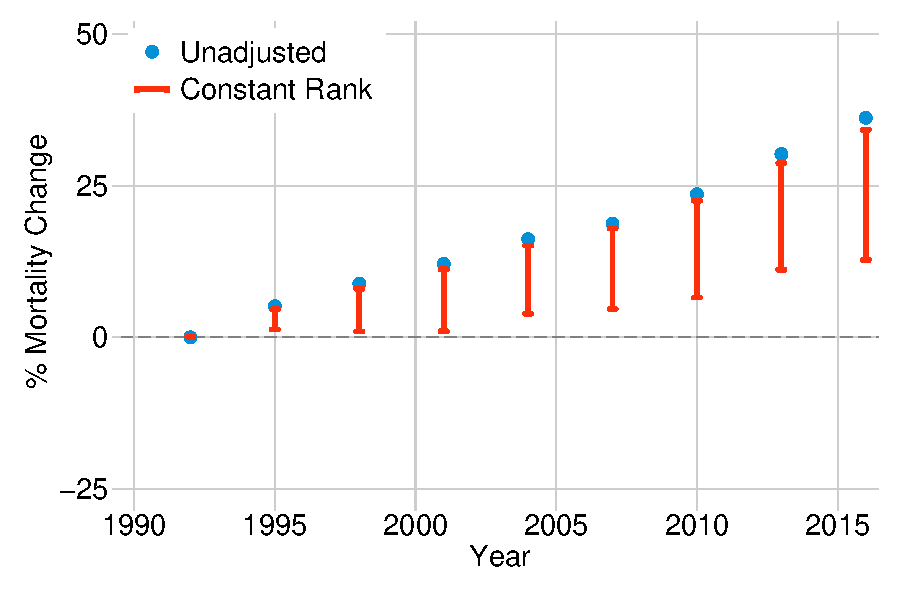
\includegraphics[scale=0.6]{\mortalitypath/naive-5-women-50-t-1} \\
      
      \panel\textbf{B. High School Completers vs. Ranks 11--45} \\
      
      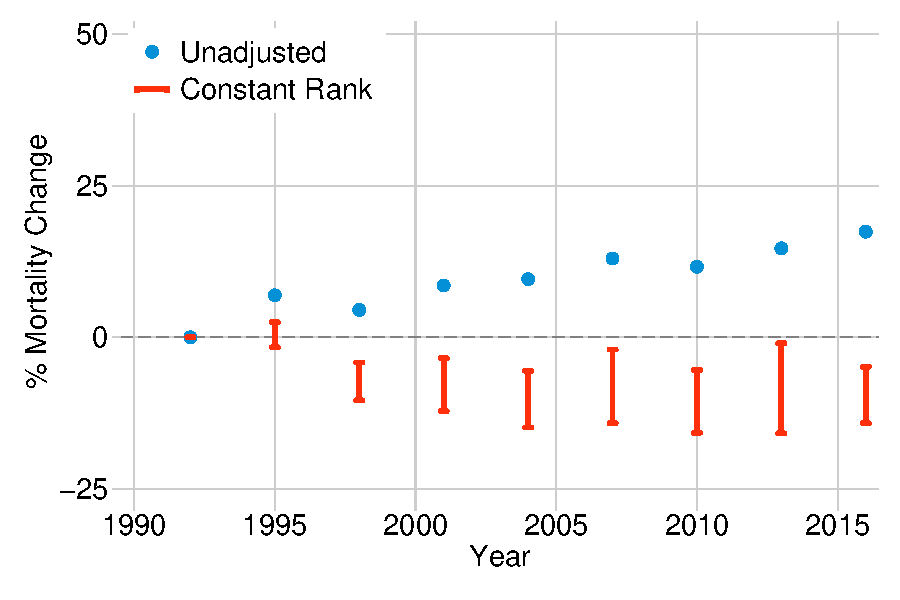
\includegraphics[scale=0.6]{\mortalitypath/naive-5-women-50-t-2} \\
    \end{tabular}
  \end{center}
  \footnotesize
  Figure~\ref{fig:naive_vs_bounds} shows mortality changes for 50--54-year-old women from 1992--94 to 2016--18 (all races combined), calculated under different methods. The points show unadjusted estimates for women at constant education levels---dropouts in Panel A and high school graduates in Panel B. Both of these population groups have shrunk as proportions of the population during the sample period. The vertical bars show bounds on mortality change in constant rank bins---ranks 0--10 in Panel A and ranks 11--45 in Panel B.
  \label{fig:naive_vs_bounds}
\end{figure}




\end{document}
